%%%%%%%%%%%%%%%%%%%%%%%%%%%%%%
%			COMMENT						
%%%%%%%%%%%%%%%%%%%%%%%%%%%%%%



\begin{comment}

Intro should stress: 
1. why the characterizazion of TJMP2 is so important for the upgrade project (OBELIX will have the same matrix analog/readout of TJMP2 + changes in the periphery to implement the trigger logic and memories for application in Belle II)
%2. what we have done in Pisa (see below) 

%3. The chip used in the DESY TestBeam was fully characterized in Pisa: TOT calibration with internal charge injection & with radioactive sources 🡪  important inputs used in TB data reconstruction and in the simulation SW of the upgraded VTX with MAPS
4. Explored also different registers settings to operate the chip with lower THResholds
 	- important after radiation damage to run at low THR to keep the hit efficiency high
5. Discovered & investigated an important issue with cross talk, due to digital signal from the redout, showing up when running the chip with THR below ~ 250 e- 
hot pixel studied to understand which digital signal was responsible & mitigate the effect with different settings/bias



Sections of this chapter could be: 
1. Matrix and flavour
2. Threshold and noise: 
	S curve internal injection, results with TB settings
	Threshold dispersion and tuning 
	Results from measurements done later (Ludovico talk TREDI) 
3. TOT calibration with internal injection 
	Also add the issue with injection circuit but not too much emphasis. 
4. Response to radioactive source and absolute calibration
5. Operation with low threshold 
	Explain the function of the various registers used (see Eleonora thesis, and maybe can add also some scope picture). 
	Register optimization 
	Comparison with simulation 
	Can add at the end some nice picture of the optimized thr and tuning 
6. Cross talk issue and mitigation 
	Description of the issue tests done and plans to mitigate it in OBELIX
7. TB June 2022 results
	prospettive del TB 2023
\end{comment}

%%%%%DRAWBACK!
%%%%%AFOREMENTIONED
%%%%%SHORTCOMINGS

\begin{comment}
%%%%%DC/AC COUPLED TO CHARGE COLLECTION ELECTRODE
Normal/Cascode differ only by one transistor designed to increase gain

Voltage step applied trough injection capacitor
\end{comment}







%%%%%%%%%%%%%%%%%%%%%%%%%%%%%%
%			COMMENT	AFT					
%%%%%%%%%%%%%%%%%%%%%%%%%%%%%%



\begin{comment}
The BCID bus width has been increased  to 7-bits because of higher gain and higher ToT slope with respect to TJ-Monopix1. \\
It's worth mentioning here that both the large column height ($\approx$ 17 mm) caused by large matrix area and the aggressive column-bus routing (which refers to the minimum line width and spacing) due to the smaller pixel size, generate a significant signal transmission delay due to the RC low pass filtering effect of the long metal wires. Consequently a special circuit has been studied that adds a variable delay to the hit pulse across the column that matches that of the BCID signal.
\end{comment}




\begin{comment}
\section{Threshold and noise} \label{thresh_noise}

In order to achieve the absolute calibration of the whole matrix, the response of each pixel has been characterized by means of the internal charge injection. \\

The hit injection circuit included in TJ-Monopix2 is similar to the one of TJ-Monopix1. It allows to inject artificial hits through an injection capacitance \textbf{$C_{inj}$} connected at the collection electrode, which is equal to 230 aF for both the DC and AC coupling FEs. The injected charge is almost linear with the injection pulse amplitude (set by the two registers ''\textbf{$V_{L}$}'' and ''\textbf{$V_{H}$}'', so that $\Delta V_{inj}$ = \textbf{$V_{H}-V_{L}$}). Moreover the injection step is finer compare to the one of TJ-Monopix1 because of the higher voltage DAC resolution, which is indeed LSB (\textit{Least Significant Bit}) = 7.03 mV. 
The injected charge resolution $Q_{res}$ can be calculated by:

\begin{equation}
\small
Q_{res} = Q_{inj} \cdot LSB= \frac{230 \, aF}{q_{{e}^{-}}} \cdot \Delta V_{inj} = 1.4375 \frac{e^{-}}{mV} \cdot 7.03 \frac{mV}{DAC \, unit} \approx 10.1 \frac{e^{-}}{DAC \, unit}  
\label{conversion_factor}
\end{equation}

Eventually this conversion factor has been used to convert the information of the injected charge from DAC unit to electrons unit, useful for further analysis.
\\
The four flavors have been separately analyzed to be able to study their main differences concerning their performance and features. The same method has been used for all of them, called \textit{s-curve method} and explained below. 


%--------------------------------------------------------------------
\subsection{S-Curve method} \label{threshold_subsection}

In order to obtain the thresold and noise values for all pixels, each one of them has to be injected an arbitrary number of times (100 times in this work) for each value of the injection pulse between a minimum voltage value, chosen setting the chip register ''\textbf{VL}'' and a maximum voltage set by the ''\textbf{VH}'' register, moving gradually with a step of 1 DAC unit (this is also adjustable). These two levels are provided by the voltage DAC.

So for each injection pulse height, the mean of 100 injection outputs are considered and it is represented as one marker in the plot.  In this way, plotting the average number of detected hits in function of the injected charge, the typical curve better known as ''\textit{S-curve}'' is reconstructed. It can be fit with the \textit{Cumulative Distribution Function (CDF)}:

\begin{equation}
 CDF(Q) = \frac{1}{2} \cdot \bigg(1 + \textit{erf}\bigg(\frac{Q-\mu}{\sigma \sqrt{2}}\bigg)\bigg)
\end{equation}

from which the value of the threshold is evaluated considering the value of the injected charge at half of the curve's maximum height. Specifically the half height corresponds to a charge value for which the pixel detects 50 hits of 100 injected and so when it has an occupancy of 0.5. This information is represented by the parameter $\mu$ obtained from the fit and the noise is evaluated from the fit parameter $\sigma$. The ''\textit{erf(x)}'' is the Gauss error function.  In figure \vref{ex_scurve} is shown an example. \\

This method allows to study the noise and threshold of all pixels and also the threshold dispersion across an entire FE.


\begin{figure}
\centering
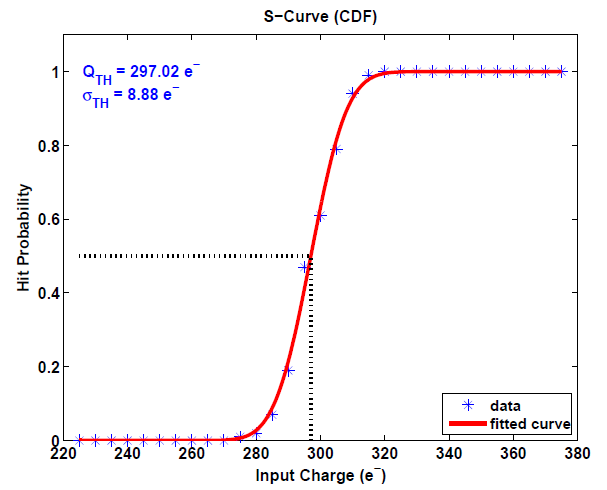
\includegraphics[scale=.6]{scurve_ex}
\caption{An example of the S-Curve fitted by the CDF to evaluate threshold and noise.}
\label{ex_scurve}
\end{figure}

In the following are reported the results of this study for the flavors of all matrix, gradually injecting a charge from 0 to 140 DAC ($\approx$ 1414 $e^{-}$ adopting the conversion factor in equation \ref{conversion_factor})


%THRESHOLD PATTERN EACH 32
%NOISE PATTERN UP DOWN
\end{comment}


\begin{comment}
\begin{table}[h!]
\centering
\begin{tabular}{>{\columncolor{ProcessBlue!60}} C{3.2cm}|C{3.7cm}|C{3.5cm}}
\rowcolor{lightgray}
Registers & Normal/Cascode FE ($P_{SUB}$/$P_{WELL}$ = -3 V) & HV/HV-Cascode FE ($P_{SUB}$/$P_{WELL}$ = 0 V, HV = +5 V)\\[2ex]
\hline
$I_{THR}$ & 64 & 30\\[0.5ex]
\hline
$I_{BIAS}$ & 50 & 60\\
\hline
$V_{RESET}$ & 143 & 100\\
\hline
$I_{CASN}$ & 0 & 8\\
\hline
$V_{CASP}$ & 93 &40\\
\hline
$V_{CASC}$ & 228 & 228\\
\hline
$I_{DB}$ & 100 & 100\\
\hline
$I_{TUNE}$ & 53 & 53\\
\hline
$V_{CLIP}$ & 255 &255\\
\hline
$I_{COMP}$ & 80 & 80\\
\hline
$I_{DEL}$ & 88 & 88\\
\hline
$I_{RAM}$ & 50 & 50\\
\hline
\end{tabular}
\caption{Settings of the main registers used for all flavors (W14R12 chip) during the Test Beam in Desy.}
\label{tab:tb_settings}
\end{table}
\end{comment}

\begin{comment}
As a matter of fact the height of the injection pulse is expected to grow linearly increasing the value of charge to be injected.
It actually happened up to a value of (about) $\approx$ 140 DAC, but for higher quantities the circuit seemed to increase not only the height of the signal, but also the threshold by a certain amount of $\Delta V$ (or equivalently of $\Delta Q$, related by the conversion factor \vpageref{conversion_factor}). Moreover, for injection heights grater than 200 DAC, only the threshold grows, without increasing the actual injected charge in any way.\\
However as we have seen in the previous section, the threshold depends on the settings of the chip registers and it can't be influenced by the injected charge, otherwise the whole response of the chip would be chaotic and it would not be reliable to take precise measurement of the impinging particles. \\

The characterization of the function used to describe the $Q_{inj}$ - ToT relationship has allowed also to extrapolate ToT values in the forbidden region of charge (above $\approx$ 1717 $e^{-}$), where the emission peaks of the radioactive sources available in the laboratory (usually) are.
\end{comment}



\begin{comment}

\begin{table}[h!]
\centering
\begin{tabular}{>{\columncolor{NavyBlue!70}} C{2.8cm}|C{1.7cm}|C{1.8cm}|C{1.7cm}|C{1.7cm}}
\rowcolor{CornflowerBlue}
Source peak & $K_{Normal}$ & $K_{Cascode}$ & $C_{HV Cascode}$ & $C_{HV}$\\[2ex]
\hline
\ch{^{55}Fe} (5.9 KeV) & 9.37 & 9.00 & 19.33 & 18.56 \\[0.5ex]
\hline
\ch{^{241}Am} (13.9 KeV) & 8.94 & 8.91 & 19.23 & 18.22 \\[0.5ex]
\hline
\ch{^{241}Am} (17.7 KeV) & 9.16 & 8.84 & 19.59 & 18.63 \\[0.5ex]
\hline
\ch{^{241}Am} (20.7 KeV) & 9.15 & 10.11 & - & -\\[0.5ex]
\hline
\ch{^{109}Cd} (22 KeV) & 9.32 & 9.39 & 20.16 & 19.6 \\[0.5ex]
\hline
\ch{^{241}Am} (26.4 KeV) & 9.60 & 9.61 & 19.25 & - \\[1.5ex]
\hline
\cellcolor{ForestGreen!80}Mean value & 9.26 & 9.31 & 19.51 & 18.75 \\[1.5ex]
\end{tabular}
\caption{Estimation of injection capacitance of all flavors for different source emission peaks.}
\label{tab:cap_mean}
\end{table}

\end{comment}


\begin{comment}
Eventually, the values of all emission peaks (obtained by the fit) from the several sources have been plotted for each frontend, in order to verify the agreement between their trend and the ToT-Q relationship studied by the internal injection. \\

\begin{figure}[h!]
\centering
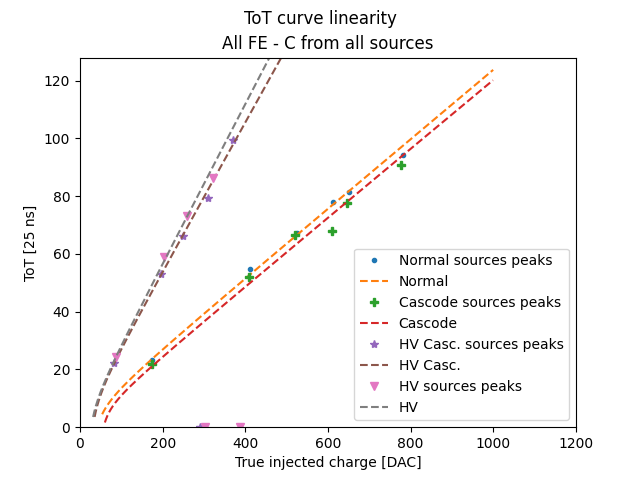
\includegraphics[scale=0.6]{Tot_linearity__sources}
\caption{Summary of trends.}
\label{inj_cap_sum}
\end{figure}
\end{comment}


\begin{comment}
In~\autoref{ch:CMOS} we have seen the fundamental steps that had lead to the development of the CMOS MAPS sensors technology, employed in the design of TJ-Monopix2.\\
\end{comment}


%[Pixel masking is also improved by employing individual in-pixel configuration memory that eliminates the issue of unintentionally masked ghost pixels and allows for a more efficient configuration of the pixel matrix and reduced noise hit rate.]

\begin{comment}
Two different token signals are used to set the priority of the pixels during the readout: the \textit{fast} one that propagates across the double column estabilishing the priority between the cores and the \textit{local} one, which arbitrates the reading order of the four pixels inside each core.
\end{comment}



\begin{comment}
In more details, there are three step for tuning:

\begin{itemize}
\item launch a first threshold scan through the internal charge injection, with a TDAC value equal for all pixels (usually default value is TDAC= 4).
\item start a TDAC analysis which allows to choose a target threshold. During this phase, a tool tries to assign the optimized value of TDAC at each pixel in several steps, in order to get as close as possible to the set threshold. At the end it returns the final TDAC values for all selected pixels.
\item At last another scan is launched setting the TDAC of each pixel passing the TDAC map values obtained from the previous. 
\end{itemize}
\end{comment}

\begin{comment}
and all of them are designed with a reduced deep p-well geometry (RDPW) because, as it was demonstrated during the testing of TJ-Monopix1, this type of arrangement has superior charge collection properties compared to full deep p-well coverage (FDPW) (\autoref{fig:tj1pix_cov}).

\begin{figure}[h!]
\centering
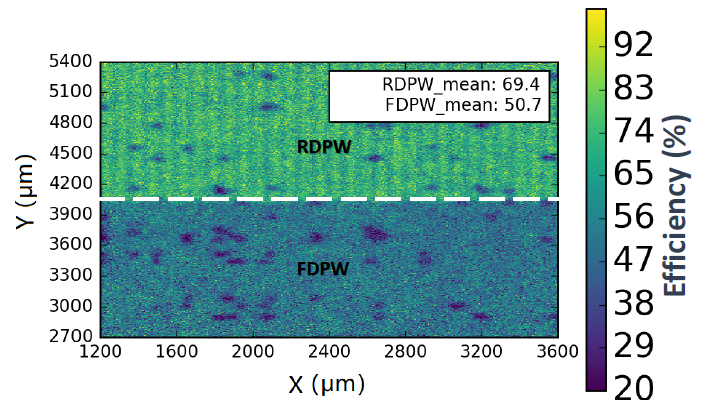
\includegraphics[scale=.6]{Tj1pix_cov}
\caption{Detection efficiency map of a TJ-Monopix1 chip with \SI{25}{\micro m} p-epitaxial layer that has been irradiated to \SI{e15}{n_{\textit{eq}}/cm^{2}} NIEL.}
\label{fig:tj1pix_cov}
\end{figure}

\end{comment}



































\begin{comment}

The ultimate purpose of this measurement is to describe (characterize) the response of each pixel by injecting a charge equivalent to the typical energy released from particles emitted in decays of radioactive materials. As explained in the previous section (reference), for example the \ch{^{55}Fe} has an emission spectrum with quite sharp lines and this allows to compare data more easily. The first line is at 5.9 KeV which corresponds on average to about 1616 $e^{-}$ released (through the pixel??).

\begin{figure}[h!]
\centering
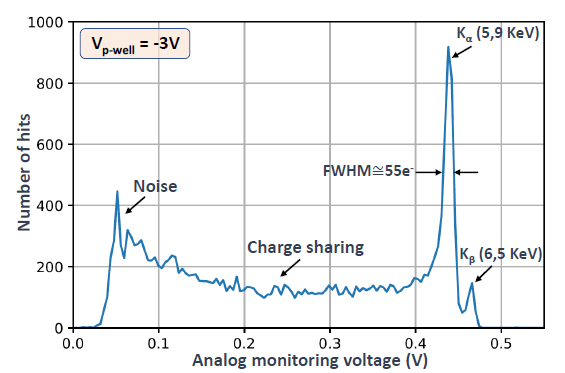
\includegraphics[scale=0.8]{spectrum_fe}
\caption{\ch{^{55}Fe} (radioactive source) emission spectrum using the analog output of a PMOS reset front-end of TJ-Monopix1. (reference)}
\label{fig:fespectrum}
\end{figure}

\end{comment}

\begin{comment}
\subsubsection{$V_{CASP}$}

[Explain VCASP]

In order to enhance this type of analysis, other scans have been run increasing the value of $V_{CASP}$ from 3 to 143, with a step of 10 DAC unit. In figure \vref{fig:th_vs_casp} the threshold's trend with respect to different values of this register.

\begin{figure}[h!]
\centering
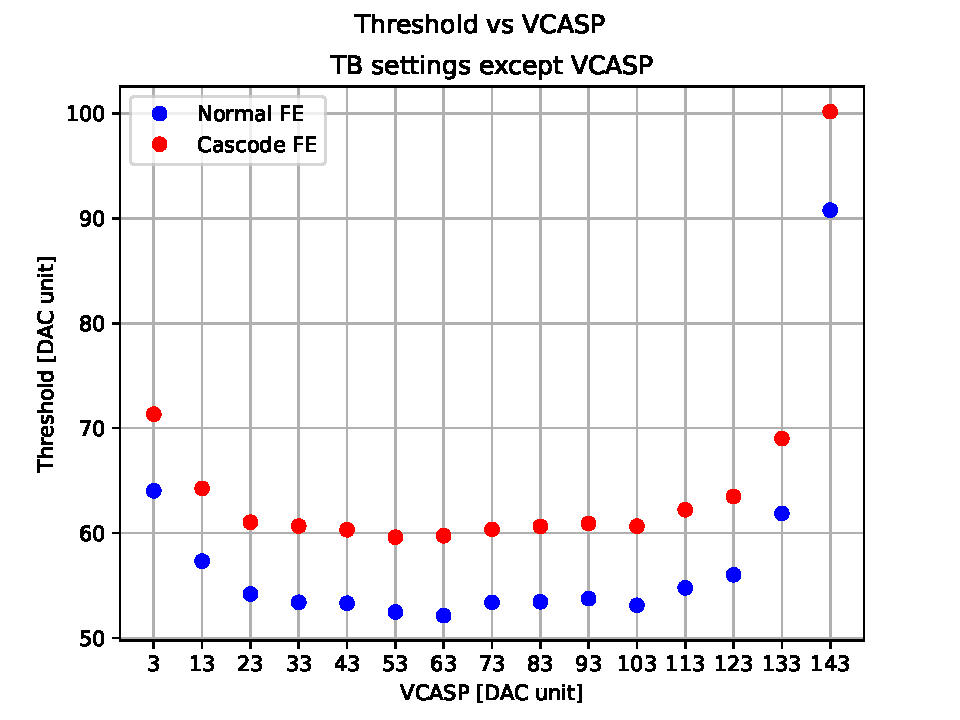
\includegraphics[scale=.7]{TH_vs_VCASP(point)}
\caption{Trends of Threshold increasing $V_{CASP}$.}
\label{fig:th_vs_casp}
\end{figure}
\end{comment}


\begin{comment}
\begin{figure}[h!]
\centering
\subfigure[VH = 140 DAC]
{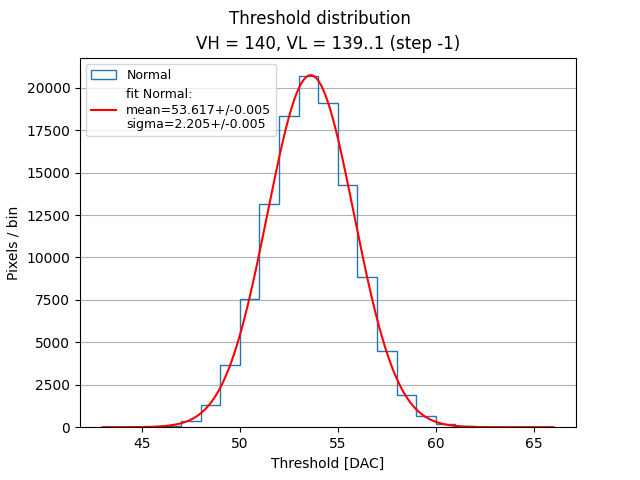
\includegraphics[scale=0.6]{all_norm_thdist_140}}\quad
\subfigure[VH = 200 DAC]
{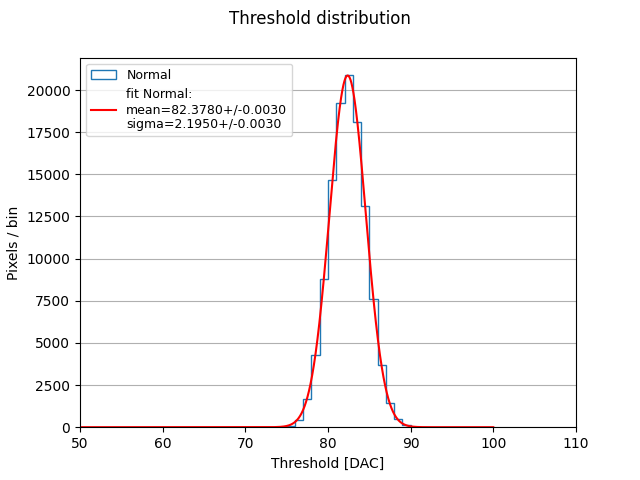
\includegraphics[scale=0.6]{all_norm_thdist_200}}\\
\caption{Threshold distributions of \textbf{Normal} flavor before and at the maximum saturation, respectively.}
\label{fig:thdist_norm}
\end{figure}

\begin{figure}[h!]
\centering
\subfigure[VH = 140 DAC]
{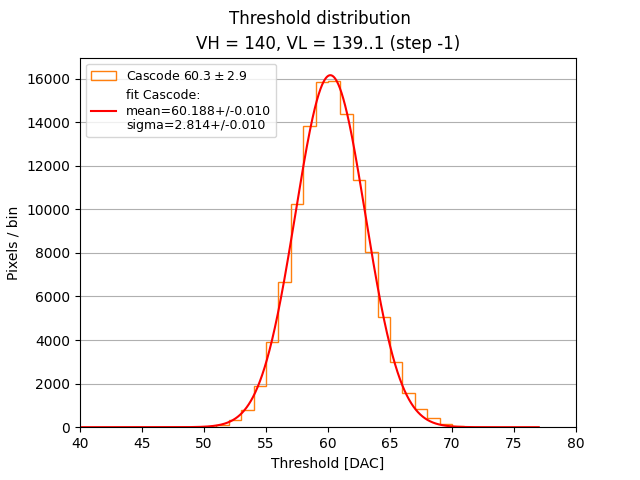
\includegraphics[scale=0.5]{all_casc_thdist_140}}\quad
\subfigure[VH = 200 DAC]
{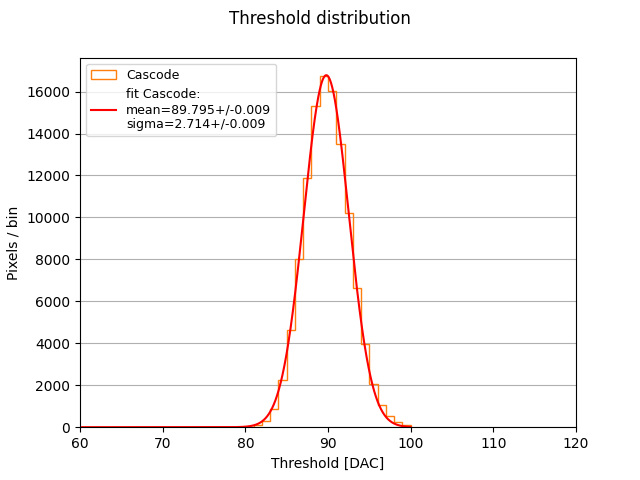
\includegraphics[scale=0.5]{all_casc_thdist_200}}\\
\caption{Threshold distributions of \textbf{Cascode} flavor before and at the maximum saturation, respectively.}
\label{fig:thdist_casc}
\end{figure}

\begin{figure}[h!]
\centering
\subfigure[VH = 140 DAC]
{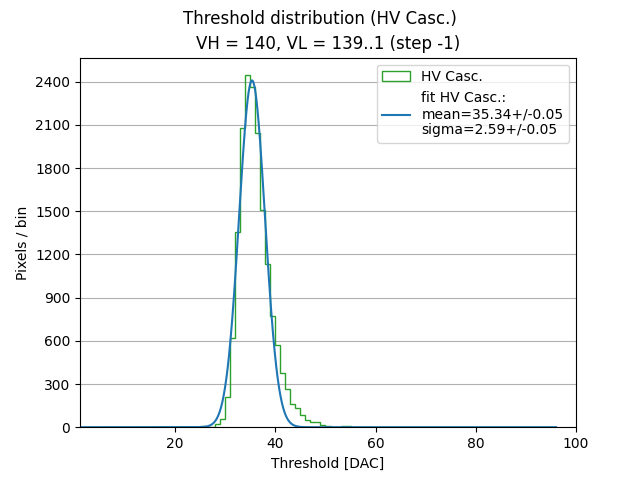
\includegraphics[scale=0.5]{all_HVc_thdist_140}}\quad
\subfigure[VH = 200 DAC]
{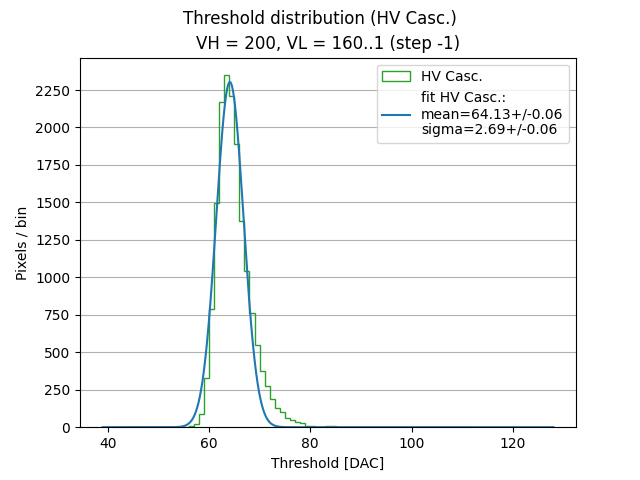
\includegraphics[scale=0.5]{all_HVc_thdist_200}}\\
\caption{Threshold distributions of \textbf{HV Cascode} flavor before and at the maximum saturation, respectively.}
\label{fig:thdist_hvc}
\end{figure}

\begin{figure}[h!]
\centering
\subfigure[VH = 140 DAC]
{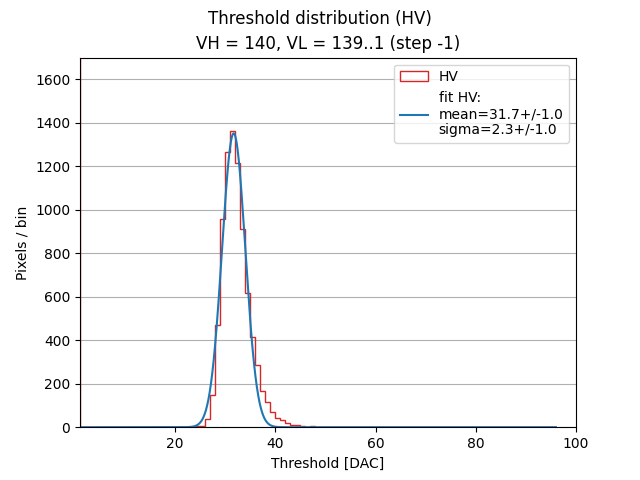
\includegraphics[scale=0.5]{all_HV_thdist_140}}\quad
\subfigure[VH = 200 DAC]
{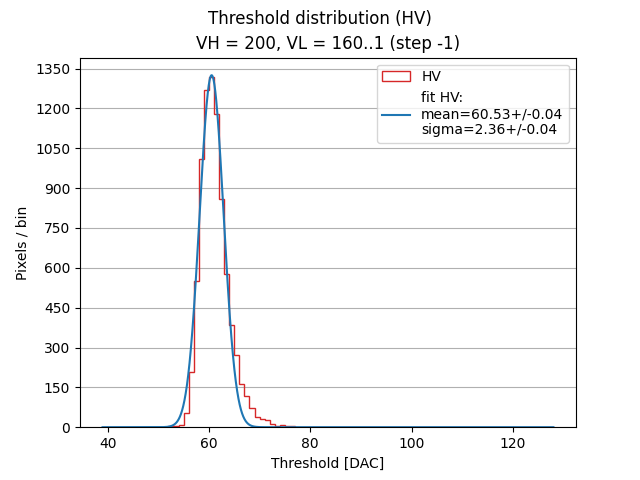
\includegraphics[scale=0.5]{all_HV_thdist_200}}\\
\caption{Threshold distributions of \textbf{HV} flavor before and at the maximum saturation, respectively.}
\label{fig:thdist_hvc}
\end{figure}
\end{comment}

%----------------------------------------------------------------------------------------------------


\begin{comment}
For the greater (higher) injection height, 8 different measurement have be actually done, each one on 28 consecutive columns and on all rows. Then data have been put together to obtain a single (summary) plot on the whole flavor. Same procedure has been preformed on the \textbf{Cascode FE}.
\end{comment}

\begin{comment}


%\subsection{Measurement of the average threshold shift for injected charge greater than 140 DAC}

To evaluate this artificial shift of the threshold, two different measurements have been done for each flavor:

\begin{itemize}
\item for an injected charge equal to 140 DAC $\rightarrow$ before the saturation region;
\item for an injected charge equal to 200 DAC $\rightarrow$ almost the maximum limit of the saturation region (from this value onward only the threshold increases, not the injected charge).
\end{itemize}

The threshold distributions obtained from each measurements have been fitted to extract an average value on the whole flavor. Naming $Q_{th, 140}$ and $Q_{th, 200}$  the threshold obtained from injections of 140 and 200 DAC respectively, the mean shift has been estimated by:

\begin{equation}
\Delta Q = Q_{th,200} - Q_{th,140}
\end{equation}

Eventually, this charge shift has been subtracted from data collected for an injection pulses of 200 DAC, in order to extrapolate the response in ToT of the injected pixels up to a value of 170 DAC.

What has been obtained is reported in the following section, together with a briefly explanation of the method used to evaluate the threshold.

\end{comment}

\begin{comment}

\begin{table}[h!]
\centering
\begin{tabular}{>{\columncolor{ProcessBlue!60}} C{3.5cm}|C{3.5cm}}
\rowcolor{lightgray}
Registri & Default Settings (''GOE'') [DAC unit]\\[2ex]
\hline
$I_{THR}$ & 64 \\[0.5ex]
\hline
$I_{BIAS}$ & 50 \\
\hline
$V_{RESET}$ & 143 \\
\hline
$I_{CASN}$ & 0 \\
\hline
$V_{CASP}$ & 93 \\
\hline
$V_{CASC}$ & 228 \\
\hline
$I_{DB}$ & 100 \\
\hline
$I_{TUNE}$ & 53 \\
\hline
$V_{CLIP}$ & 255 \\
\hline
$I_{COMP}$ & 80 \\
\hline
$I_{DEL}$ & 88 \\
\hline
$I_{RAM}$ & 50 \\
\hline
\end{tabular}
\caption{Settings of the main registers used for the W14R12 chip, for Normal and Cascode flavors, during the Test Beam in Desy.}
\label{tab:tb_settings}
\end{table}

\begin{table}[h!]
\centering
\begin{tabular}{>{\columncolor{Green!60}} C{3.5cm}|C{3.5cm}}
\rowcolor{lightgray}
Registri & Default Settings (''GOE'') [DAC unit]\\
\hline
$I_{THR}$ & 30 \\
\hline
$I_{BIAS}$ & 60 \\
\hline
$V_{RESET}$ & 100 \\
\hline
$I_{CASN}$ & 8 \\
\hline
$V_{CASP}$ & 40 \\
\hline
$V_{CASC}$ & 228 \\
\hline
$I_{DB}$ & 100 \\
\hline
$I_{TUNE}$ & 53 \\
\hline
$V_{CLIP}$ & 255 \\
\hline
$I_{COMP}$ & 80 \\
\hline
$I_{DEL}$ & 88 \\
\hline
$I_{RAM}$ & 50 \\
\hline
\end{tabular}
\caption{Settings of the main registers used for the W14R12 chip, for the HV's flavors, during the Test Beam in Desy.}
\label{tab:tb_hv_settings}
\end{table}
\end{comment}

\begin{comment}
\begin{figure}[h!]
\centering
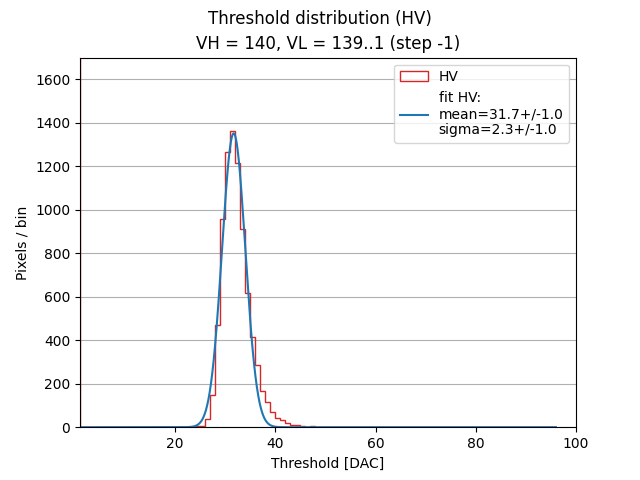
\includegraphics[scale=0.5]{all_HV_thdist_140}
\caption{Threshold distributions of \textbf{HV} flavor for VH = 140 DAC}
\label{fig:thdist_hv}
\end{figure}
\end{comment}

\begin{comment}
\begin{figure}[h!]
\centering
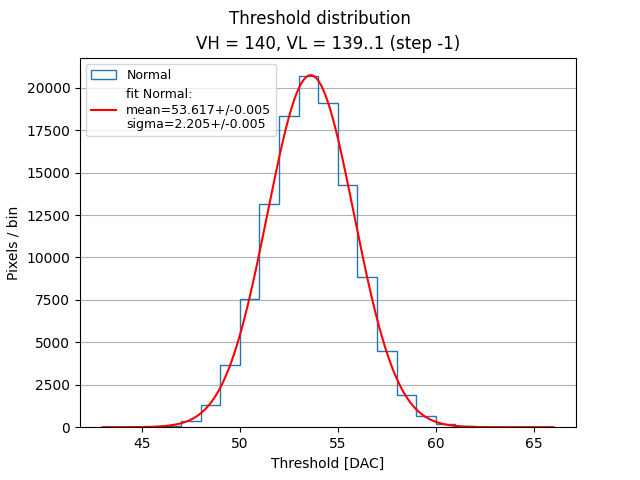
\includegraphics[scale=0.5]{all_norm_thdist_140}
\caption{Threshold distributions of \textbf{Normal} flavor for VH = 140 DAC}
\label{fig:thdist_norm}
\end{figure}
\end{comment}

\begin{comment}
\begin{figure}[h!]
\centering
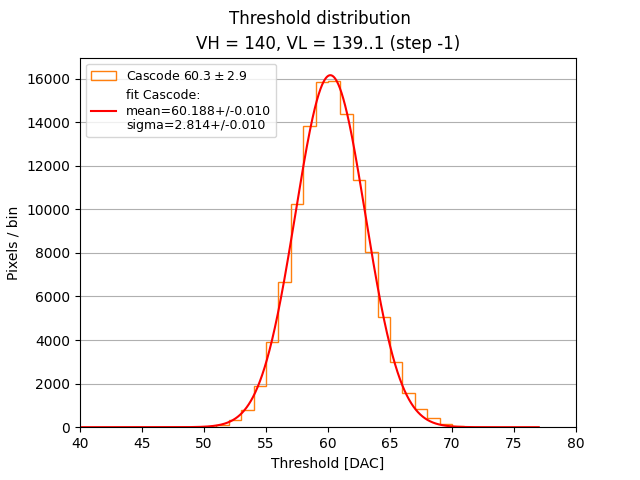
\includegraphics[scale=0.5]{all_casc_thdist_140}
\caption{Threshold distributions of \textbf{Cascode} flavor for VH = 140 DAC.}
\label{fig:thdist_casc}
\end{figure}
\end{comment}

\begin{comment}
\begin{figure}[h!]
\centering
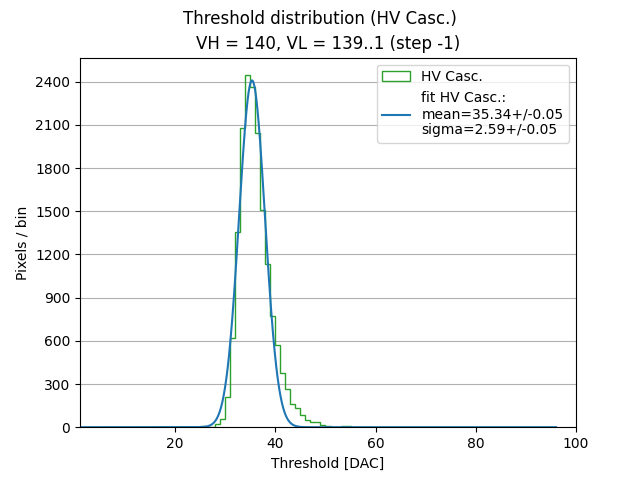
\includegraphics[scale=.5]{all_HVc_thdist_140}
\caption{Threshold distributions of \textbf{HV Cascode} flavor for VH = 140 DAC.}
\label{fig:thdist_hvc}
\end{figure}
\end{comment}

\begin{comment}
In the last plots of this section (\vpageref{fig:tot_vs_vcasp}) are reported the trends of the ToT varying the value of $V_{CASP}$ for both Normal and Cascode FE, but there aren't simulations to make a comparison. 

\begin{figure}[h!]
\centering
\subfigure[ToT vs $V_{CASP}$ - Data (\textbf{Cascode})]
{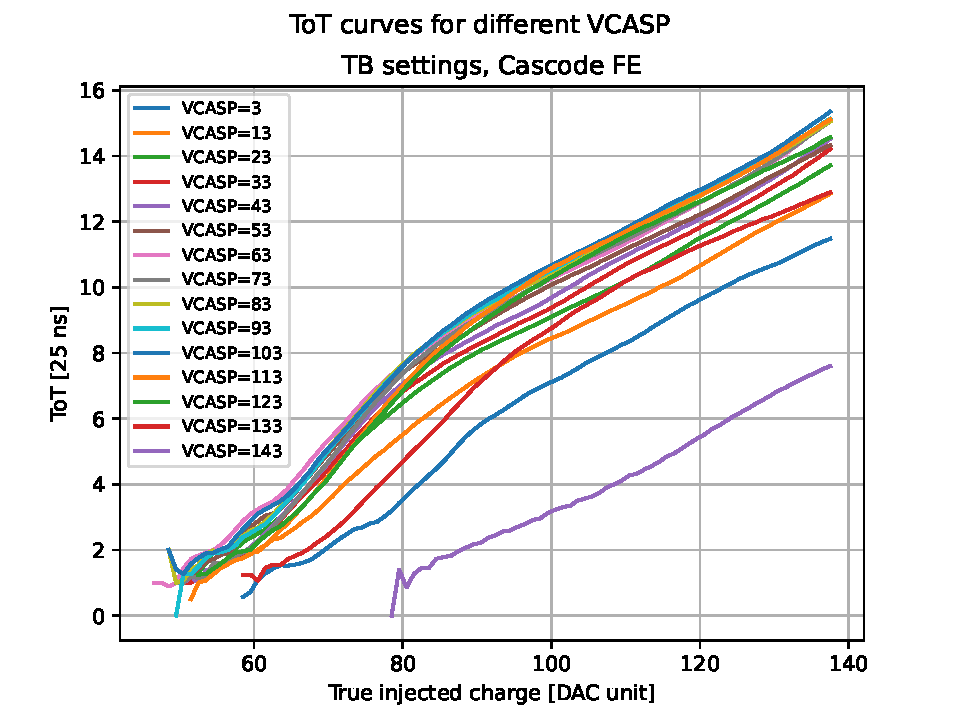
\includegraphics[scale=0.4]{tot_vcasp(cascode)}}\quad
\subfigure[ToT vs $V_{CASP}$ - Data (\textbf{Normal})]
{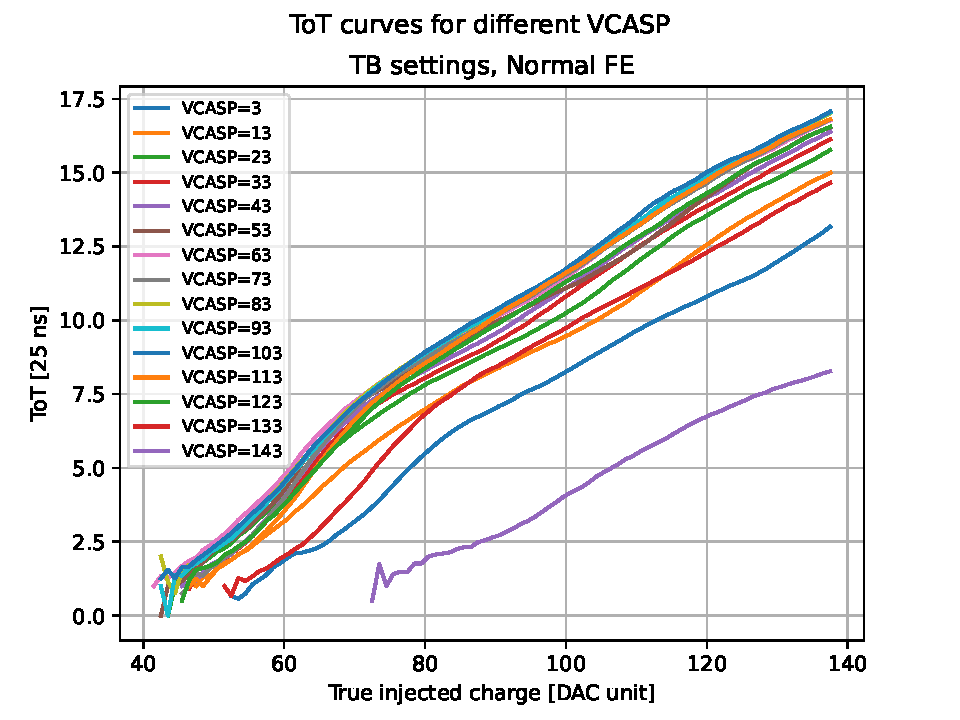
\includegraphics[scale=0.4]{tot_vcasp(normal)}}\\
\caption{ToT vs $V_{CASP}$}
\label{fig:tot_vs_vcasp}
\end{figure}
\end{comment}


\begin{comment}
\begin{itemize}
\item[$I_{THR}=64$]:

\begin{tabular}{c | c | c}
$I_{CASN}$ [DAC] & THR [DAC] & THR Dispersion [DAC]\\
\hline
0 & 61.43 & 2.45\\
5 & 53.42 & 2.45\\
10 & 50.33 & 2.45\\
15 & 48.21 & 2.41\\
20 & 46.70 & 2.38\\
25 & 45.49 & 2.52\\
30 & 46.09 & 2.50
\end{tabular}

\item[$I_{THR}=40$]:

\begin{tabular}{c | c | c}
$I_{CASN}$ [DAC] & THR [DAC] & THR Dispersion [DAC]\\
\hline
0 & 47.28 & 2.12\\
5 & 41.07 & 2.02\\
10 & 38.39 & 2.03\\
15 & 36.65 & 1.95\\
20 & 35.53 & 1.91\\
25 & NaN & NaN\\
30 & 33.37 & 2.04
\end{tabular}

[Here we can see a particular setting, that is $I_{THR}=40$ AND $I_{CASN}$=25, for which the chip doesn't seem to work.
PIXEL THAT FIRE UP??]

\item[$I_{THR}=20$]:

\begin{tabular}{c | c | c}
$I_{CASN}$ [DAC] & THR [DAC] & THR Dispersion [DAC]\\
\hline
0 & 34.43 & 1.95\\
5 & 28.10& 1.72\\
10 & 26.59 & 1.75\\
15 & 24.66 & 1.77\\
\end{tabular}
\medskip\\

\end{itemize}
\end{comment}

\begin{comment}
During this study an iportant issue with cross-talk(readout signal) was discovered. As it was already mentioned, also in the threshold analysis for the HVs flavors, there were something atypical in the s-curves, because some of them seem to have occupancy greater than 1!
So in this section we will go through this effect and some attempt to mitigate the effect using different settings/bias. 

\end{comment}